\documentclass[a4paper,12pt]{article}
%%% Default imports
\usepackage{listings} % Code listings
\usepackage{graphicx} % Images
\usepackage{booktabs} % Better tables
\usepackage{makecell}
\usepackage{enumitem} % Lists
\usepackage{dsfont}
\usepackage{geometry} % Page geometry
\usepackage[utf8]{inputenc} % Encoding
\usepackage[T2A]{fontenc} % Font
\usepackage[english, russian]{babel} % Multi-language support
\usepackage{titling} % Better titles
\usepackage{textcomp} % Old-style numbers? Check difference
\usepackage{mathtext} % Russian text in math expressions? Check difference
\usepackage{amsmath, amsfonts, amssymb, amsthm, mathtools} % Mathematics
\usepackage{bm} % Bold math symbols
\usepackage{icomma} % Better comma in numbers within math mode
\usepackage{xifthen} % Better if-expressions
\usepackage{transparent} % Transparent colors
\usepackage{caption}    % }
\usepackage{subcaption} % } Captioning figures
\usepackage[table,xcdraw]{xcolor} % Colors
\usepackage{textpos} % Absolute positioning
\usepackage{upgreek} % Cool greek letters

\usepackage{fancyvrb}
\usepackage{fvextra}
\usepackage{chngcntr}

%%% Page geometry
\setlength\parindent{0pt} % No indentation between paragraphs
\setlist{noitemsep} % No spacing between list items

\usepackage{float}
\usepackage{multirow}

\geometry{
    paper=a4paper,
    top=2.5cm,
    bottom=3cm,
    left=2.5cm,
    right=2.5cm,
    headheight=0.75cm,
    footskip=1.5cm,
    headsep=0.75cm,
}

%%% Numeration
\newcommand{\RNumb}[1]{\uppercase\expandafter{\romannumeral #1\relax}}
\newcommand{\thesec}{\arabic{section}}
\renewcommand\thesection{\arabic{section}}
\renewcommand\thesubsection{\thesection.\arabic{subsection}}
\renewcommand\thesubsubsection{\RNumb{\arabic{subsubsection}}}
\renewcommand{\sectionmark}[1]{\markright{\thesection\ #1}}
\renewcommand{\bf}{\textbf}
\renewcommand{\it}{\textit}
\def\hash{\texttt{\#}}
\def\cpp{\C\texttt{++}}

\counterwithin{figure}{section}
\counterwithin{table}{section}
\renewenvironment{titlepage}{\thispagestyle{empty}} % Include titlepage into page numeration

%%% Headers and footers
\usepackage{setspace}
\usepackage{fancyhdr}
\usepackage{lastpage}


%%% Graphics
% Custom colors
\definecolor{myblue}{RGB}{72, 184, 178}
\definecolor{myblue1}{RGB}{0, 109, 167}
\definecolor{commentgreen}{RGB}{2,112,10}
\definecolor{mauve}{rgb}{0.58,0,0.82}
\definecolor{amethyst}{RGB}{153, 102, 203}

\usepackage{pgfplots} % Plots
\usepackage{tikz}
\usetikzlibrary{3d,perspective,decorations.text}
\usetikzlibrary{animations}
\usetikzlibrary{positioning}
\usetikzlibrary{matrix}
\usepackage{tikz-cd}
\usetikzlibrary{cd}
\usetikzlibrary{karnaugh}
\pgfplotsset{width=6cm,compat=newest}
\usepackage{color}

\usepackage[framemethod=TikZ]{mdframed}
\newcommand{\definebox}[2]{\newcounter{#1}\newenvironment{#1}[1][]{\stepcounter{#1}\mdfsetup{frametitle={\tikz[baseline=(current bounding box.east),outer sep=0pt]\node[anchor=east,rectangle,fill=white]{\strut \MakeUppercase#1~\csname the#1\endcsname\ifstrempty{##1}{}{:~##1}};}}\mdfsetup{innertopmargin=1pt,linecolor=#2,linewidth=3pt,topline=true,frametitleaboveskip=\dimexpr-\ht\strutbox\relax,}\begin{mdframed}[]\relax}{\end{mdframed}}}
\definebox{definition}{black!90}
\definebox{theorem}{myblue1!90}
\definebox{demonstration}{amethyst!90}

\newcounter{Theorem}
\def\themytheorem{\thesection.\arabic{Theorem}}
\usepackage[most]{tcolorbox}
\tcbuselibrary{theorems}
\newtcbtheorem{Theorem}{Theorem}
{colframe=myblue!90,coltitle=black,colback=white,fonttitle=\bfseries}{Th}

%%% Code listings
\usepackage{matlab-prettifier}

\lstdefinestyle{cpp} {
    language=C++,
    frame=tb,
    tabsize=4,
    showstringspaces=false,
    numbers=left,
    captionpos=b,
    columns=flexible,
    upquote=true,
    commentstyle=\color{commentgreen},
    keywordstyle=\color{blue},
    stringstyle=\color{commentgreen},
    basicstyle=\small\ttfamily,
    emph={int,char,double,float,unsigned,void,bool,size\_t},
    emphstyle={\color{blue}},
    escapechar=\&,
    classoffset=1,
    otherkeywords={>,<,.,;,-,!,=,~},
    morekeywords={>,<,.,;,-,!,=,~},
    keywordstyle=\color{black},
    classoffset=0,
}
\lstdefinestyle{def} {
    frame=tb,
    tabsize=4,
    showstringspaces=false,
    numbers=left,
    captionpos=b,
    columns=flexible,
    upquote=true,
    commentstyle=\color{black},
    keywordstyle=\color{black},
    stringstyle=\color{black},
    basicstyle=\small\ttfamily,
    emph={int,char,double,float,unsigned,void,bool,size\_t},
    emphstyle={\color{black}},
    escapechar=\&,
    classoffset=1,
    otherkeywords={>,<,.,;,-,!,=,~},
    morekeywords={>,<,.,;,-,!,=,~},
    keywordstyle=\color{black},
    classoffset=0,
}
\lstdefinelanguage[RISC-V]{Assembler}
{
    alsoletter={.}, % allow dots in keywords
    alsodigit={0x}, % hex numbers are numbers too!
    morekeywords=[1]{ % instructions
    lb, lh, lw, lbu, lhu,
    sb, sh, sw,
    sll, slli, srl, srli, sra, srai,
    add, addi, sub, lui, auipc,
    xor, xori, or, ori, and, andi,
    slt, slti, sltu, sltiu,
    beq, bne, blt, bge, bltu, bgeu,
    j, jr, jal, jalr, ret,
    scall, break, nop
},
    morekeywords=[2]{ % sections of our code and other directives
    .align, .ascii, .asciiz, .byte, .data, .double, .extern,
    .float, .globl, .half, .kdata, .ktext, .set, .space, .text, .word
},
    morekeywords=[3]{ % registers
    zero, ra, sp, gp, tp, s0, fp,
    t0, t1, t2, t3, t4, t5, t6,
    s1, s2, s3, s4, s5, s6, s7, s8, s9, s10, s11,
    a0, a1, a2, a3, a4, a5, a6, a7,
    ft0, ft1, ft2, ft3, ft4, ft5, ft6, ft7,
    fs0, fs1, fs2, fs3, fs4, fs5, fs6, fs7, fs8, fs9, fs10, fs11,
    fa0, fa1, fa2, fa3, fa4, fa5, fa6, fa7
},
    morecomment=[l]{;},   % mark ; as line comment start
    morecomment=[l]{\#},  % as well as # (even though it is unconventional)
    morestring=[b]",      % mark " as string start/end
    morestring=[b]'       % also mark ' as string start/end
}
\lstdefinestyle{riscv} {
    basicstyle=\small\ttfamily,                    % very small code
    breaklines=true,                              % break long lines
    commentstyle=\itshape\color{green!50!black},  % comments are green
    keywordstyle=[1]\color{blue!80!black},        % instructions are blue
    keywordstyle=[2]\color{orange!80!black},      % sections/other directives are orange
    keywordstyle=[3]\color{red!50!black},         % registers are red
    stringstyle=\color{mauve},                    % strings are from the telekom
    identifierstyle=\color{teal},                 % user declared addresses are teal
    frame=l,                                      % black line on the left side of code
    captionpos=b,
    language=[RISC-V]Assembler,                   % all code is RISC-V
    tabsize=4,                                    % indent tabs with 4 spaces
    showstringspaces=false                        % do not replace spaces with weird underlines
}

%%% Other
\usepackage[normalem]{ulem} % }
\useunder{\uline}{\ul}{}    % } Underline text
\usepackage[colorlinks,urlcolor=blue,filecolor=blue,citecolor=blue,linkcolor = blue,unicode=true]{hyperref}
\usepackage{titlesec}
\titlelabel{\thetitle.\quad}
\usepackage{secdot}
\sectiondot{subsection}
\usepackage{kvmap} % Karnaugh-maps for logic functions
\usepackage{}
\newcommand{\projectname}[3]{
    \begin{center}
        \Large
        \textbf{#1}\\[10pt]
        \textbf{#2}\\[10pt]
        \normalsize
        #3
        \rule{\linewidth}{0.4pt}
    \end{center}
}

\newcommand{\hfconfiguration}[3]{
    \pagestyle{fancy}
    \fancyhead[LE,RO]{}
    \fancyhead[LO,RE]{#1}
    \renewcommand{\footrulewidth}{0.4pt}
    \fancyfoot[C]{\thepage/\pageref*{LastPage}}
    \fancyfoot[LO,RE]{#2}
    \fancyfoot[LE,RO]{#3}
}

\newcommand{\filename}[2]{
    \pagebreak
    \titleformat{\section}
    [display]
    {\bfseries\Large}
    {}
    {0ex}
    {
        \vspace{-4.5ex}
        % \rule{\textwidth}{1pt}
        #1 \centering
    % \vspace{1ex}
    }
    [
        \normalfont\large
        #2
        \rule{\textwidth}{0.4pt}
        \normalsize
    ]
}

\newcommand{\project}[6]{
    \projectname{#1}{#2}{#3}
    \pagestyle{empty}
    \tableofcontents
    \newpage
    \hfconfiguration{#4}{#5}{#6}
}
%%% Final touch
\usepackage{subfiles}


\begin{document}
    \begin{titlepage}
    \begin{center}
        \large Санкт-Петербургский политехнический университет Петра Великого\\
        \large Институт компьютерных наук и технологий \\
        \large Кафедра компьютерных систем и программных технологий\\[6cm]


        \huge Отчет по лабораторной работе №3\\[0.5cm]
        \large по дисциплине <<Схемотехника операционных устройств>>\\[0.1cm]
        \large\textbf{Триггеры}\\[5cm]
    \end{center}


    \begin{flushright}
        \begin{minipage}{0.25\textwidth}
            \begin{flushleft}

                \large\textbf{Работу выполнил:}\\
                \large Ильин В.П.\\
                \large {Группа:} 35300901/10005\\

                \large \textbf{Преподаватель:}\\
                \large Киселев И.О.

            \end{flushleft}
        \end{minipage}
    \end{flushright}

    \vfill

    \begin{center}
        \large Санкт-Петербург\\
        \large \the\year
    \end{center}
\end{titlepage}

\vfill
\newpage

    % \tableofcontents
    \hfconfiguration{Лабораторная работа №3}{}{}

    \section{Цели работы}
    \begin{itemize}
        \item Закрепление знания характеристик и режимов работы триггеров основных типов;
        \item получение практических навыков тестирования и управления триггерами;
        \item получение навыков ввода проекта в графическом редакторе пакета QP, тестирования
        и отладки проекта и анализа временных характеристик триггеров;
        \item получение навыков отладки цифровых устройств данного класса на физической модели;
        конфигурирование ПЛИС и экспериментальная проверка работы типовых устройств с триггерами
        при использовании лабораторной платы DiLaB.
    \end{itemize}
    \section{Исходные данные}
    \begin{table}[H]
        \centering
        \begin{tabular}{|c|c|c|c|}
            \hline Вариант & Длительность импульса & Фронт/спад & Частота \\
            \hline 8 & 8 нс & Спад & 1.5 Гц \\
            \hline
        \end{tabular}
    \end{table}
    \section{Ход работы}
    \subsection{Асинхронный RS-триггер}

    \begin{figure}[H]
		\centering
		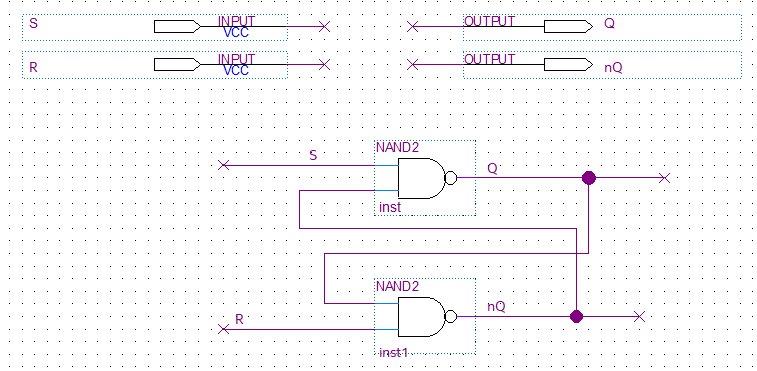
\includegraphics[width=\linewidth]{polytech/scheme/report-lab3/subfiles/images/scheme-1}
		\caption{Разработанная схема триггера}
		\label{fig:scheme-1}
	\end{figure}
    
    \begin{figure}[H]
		\centering
		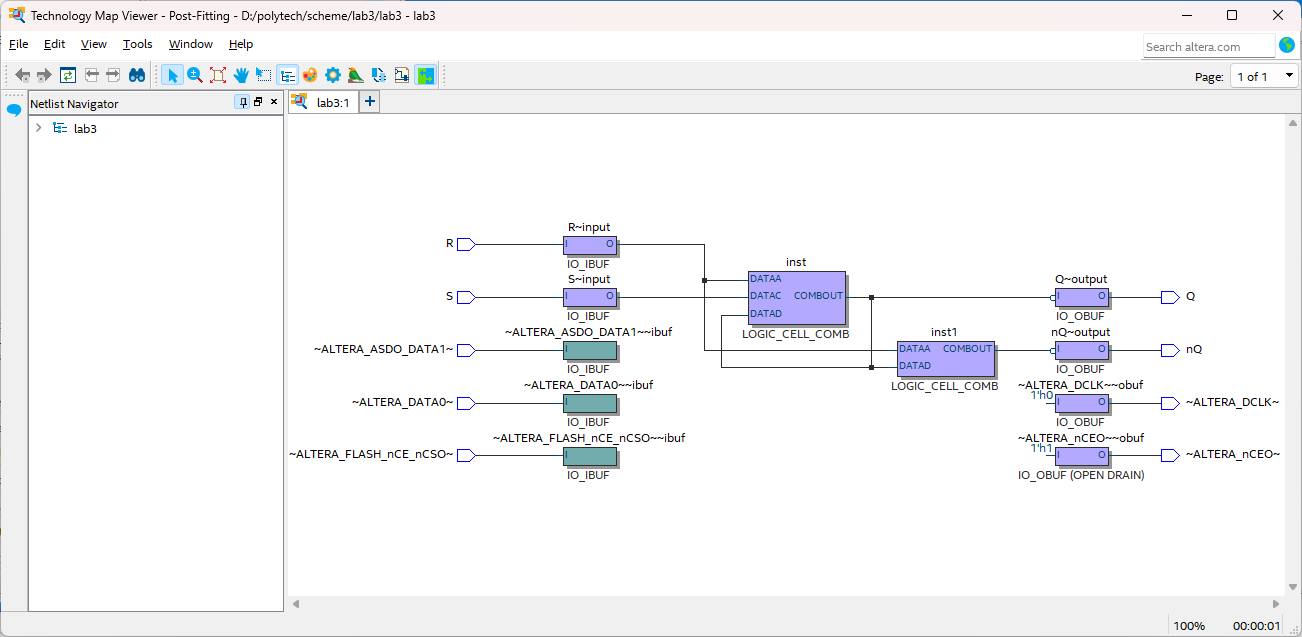
\includegraphics[width=\linewidth]{polytech/scheme/report-lab3/subfiles/images/tech-mv-1}
		\caption{Схема в Technology Map Viewer}
		\label{fig:tech-mv-1}
	\end{figure}
    
    \begin{table}[H]
        \centering
        \begin{tabular}{|c|cc|cc|c|}
        \hline
        \multirow{2}{*}{\begin{tabular}[c]{@{}c@{}}Дискретное\\ время $t$\\\end{tabular}} & \multicolumn{2}{c|}{Входные переменные} & \multicolumn{2}{c|}{Состояния}    & \multirow{2}{*}{Режим работы} \\ \cline{2-5}
                                                                                        & \multicolumn{1}{c|}{$S(t)$}     & $R(t)$    & \multicolumn{1}{c|}{$Q(t)$} & $nQ(t)$ &                               \\ \hline
        0                                                                               & \multicolumn{1}{c|}{0}        & 1       & \multicolumn{1}{c|}{1}    & 0     & Установка 1                   \\ \hline
        1                                                                               & \multicolumn{1}{c|}{1}        & 1       & \multicolumn{1}{c|}{1}    & 0     & Хранение 1                    \\ \hline
        2                                                                               & \multicolumn{1}{c|}{1}        & 0       & \multicolumn{1}{c|}{0}    & 1     & Установка 0                   \\ \hline
        3                                                                               & \multicolumn{1}{c|}{1}        & 1       & \multicolumn{1}{c|}{0}    & 1     & Хранение 0                    \\ \hline
        4                                                                               & \multicolumn{1}{c|}{0}        & 0       & \multicolumn{1}{c|}{1}    & 1     & Особое состояние                   \\ \hline
        \end{tabular}
        \caption{Таблица переходов триггера}
        \label{tab:tab-1}
    \end{table}
    
    \begin{figure}[H]
		\centering
		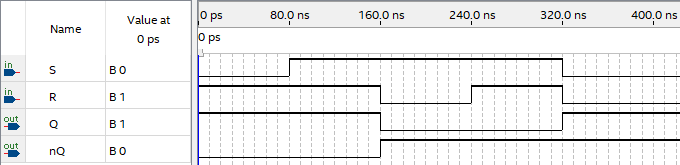
\includegraphics[width=\linewidth]{polytech/scheme/report-lab3/subfiles/images/wave-1}
		\caption{Временная диаграмма}
		\label{fig:wave-1}
	\end{figure}

    \begin{figure}[H]
		\centering
		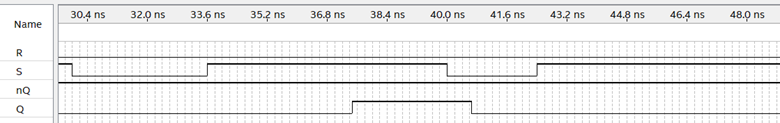
\includegraphics[width=\linewidth]{polytech/scheme/report-lab3/subfiles/images/wave-1-2}
		\caption{Временная диаграмма с импульсами}
		\label{fig:wave-1-2}
	\end{figure}
    По результатам моделирования видно, что минимальная длительность сигнала, переключающего триггер
    составляет $3.6$ нс.
    \subsection{RS-триггер синхронизируемый уровнем}
    \begin{figure}[H]
		\centering
		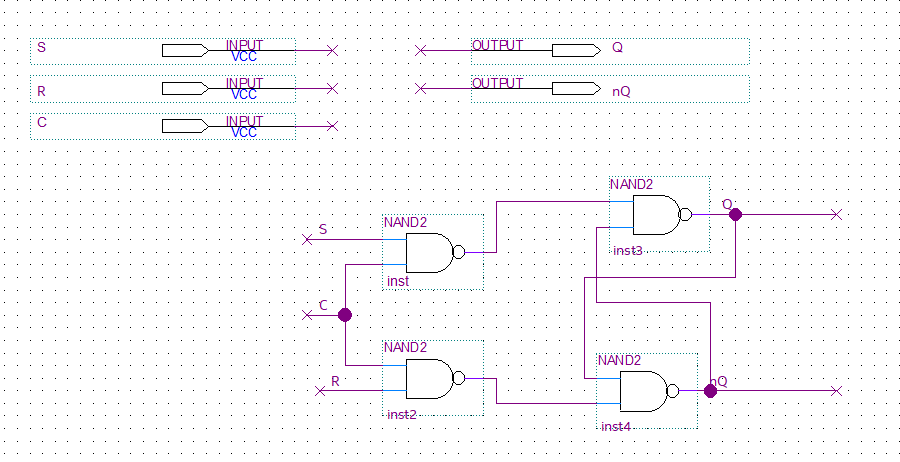
\includegraphics[width=\linewidth]{polytech/scheme/report-lab3/subfiles/images/scheme-2}
		\caption{Разработанная схема триггера}
		\label{fig:scheme-2}
	\end{figure}
    \begin{table}[H]
        \centering
        \begin{tabular}{|c|ccc|cc|c|}
        \hline
        \multirow{2}{*}{\begin{tabular}[c]{@{}c@{}}Дискретное\\ время $t$\end{tabular}} & \multicolumn{3}{c|}{Входные переменные}                            & \multicolumn{2}{c|}{Состояния}         & \multirow{2}{*}{Режим работы}     \\ \cline{2-6}
                                                                                        & \multicolumn{1}{c|}{$C(t)$} & \multicolumn{1}{c|}{$S(t)$} & $R(t)$ & \multicolumn{1}{c|}{$Q(t)$} & $Q(t+1)$ &                                   \\ \hline
        0                                                                               & \multicolumn{1}{c|}{0}      & \multicolumn{1}{c|}{H}      & H      & \multicolumn{1}{c|}{0}      & 0        & \multirow{2}{*}{Хранение}         \\ \cline{1-6}
        1                                                                               & \multicolumn{1}{c|}{0}      & \multicolumn{1}{c|}{H}      & H      & \multicolumn{1}{c|}{1}      & 1        &                                   \\ \hline
        2                                                                               & \multicolumn{1}{c|}{1}      & \multicolumn{1}{c|}{0}      & 0      & \multicolumn{1}{c|}{0}      & 0        & \multirow{2}{*}{Хранение}         \\ \cline{1-6}
        3                                                                               & \multicolumn{1}{c|}{1}      & \multicolumn{1}{c|}{0}      & 0      & \multicolumn{1}{c|}{1}      & 1        &                                   \\ \hline
        4                                                                               & \multicolumn{1}{c|}{1}      & \multicolumn{1}{c|}{1}      & 0      & \multicolumn{1}{c|}{0}      & 1        & \multirow{2}{*}{Запись 1}         \\ \cline{1-6}
        5                                                                               & \multicolumn{1}{c|}{1}      & \multicolumn{1}{c|}{1}      & 0      & \multicolumn{1}{c|}{1}      & 1        &                                   \\ \hline
        6                                                                               & \multicolumn{1}{c|}{1}      & \multicolumn{1}{c|}{0}      & 1      & \multicolumn{1}{c|}{0}      & 0        & \multirow{2}{*}{Запись 0}         \\ \cline{1-6}
        7                                                                               & \multicolumn{1}{c|}{1}      & \multicolumn{1}{c|}{0}      & 1      & \multicolumn{1}{c|}{1}      & 0        &                                   \\ \hline
        8                                                                               & \multicolumn{1}{c|}{1}      & \multicolumn{1}{c|}{1}      & 1      & \multicolumn{1}{c|}{0}      & H        & \multirow{2}{*}{Особое состояние} \\ \cline{1-6}
        9                                                                               & \multicolumn{1}{c|}{1}      & \multicolumn{1}{c|}{1}      & 1      & \multicolumn{1}{c|}{1}      & H        &                                   \\ \hline
        \end{tabular}
        \caption{Таблица переходов триггера}
        \label{tab:tab-2}
    \end{table}
    \begin{figure}[H]
		\centering
		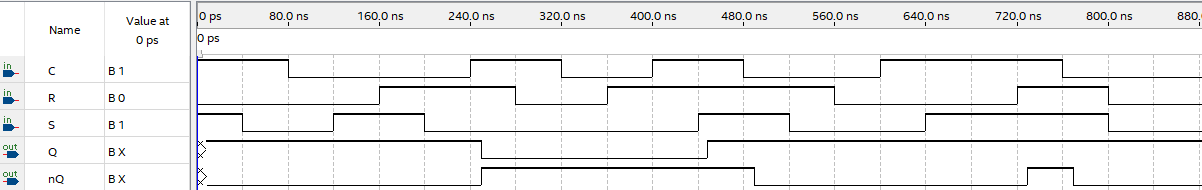
\includegraphics[width=\linewidth]{polytech/scheme/report-lab3/subfiles/images/wave-2}
		\caption{Временная диаграмма}
		\label{fig:wave-2}
	\end{figure}
    Из результатов моделирования видно, что триггер синхронизируется уровнем, а не перепадом.
    При переходе триггера из особого состояния в состояние хранения на его выходе сохраняется <<1>>.
    
    \subsection{Использование примитива DFFE}
    \begin{figure}[H]
		\centering
		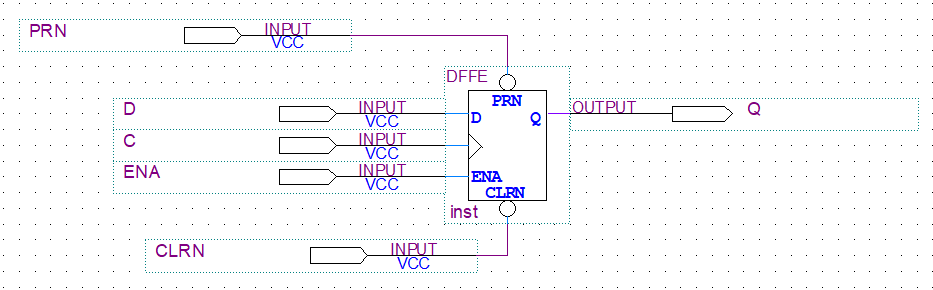
\includegraphics[width=\linewidth]{polytech/scheme/report-lab3/subfiles/images/scheme-3}
		\caption{Разработанная схема триггера}
		\label{fig:scheme-3}
	\end{figure}
    \begin{figure}[H]
		\centering
		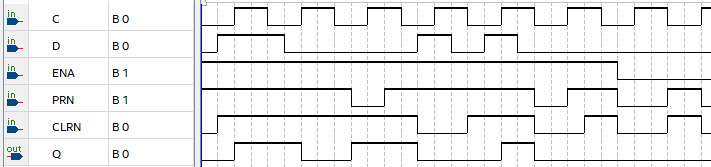
\includegraphics[width=\linewidth]{polytech/scheme/report-lab3/subfiles/images/wave-3}
		\caption{Временная диаграмма}
		\label{fig:wave-3}
	\end{figure}
    При одновременной подаче активного уровня на входы PRN и CLRN триггер устанавливается в 0.
    \subsection{Использование примитива JKFFE}
    
    \begin{figure}[H]
		\centering
		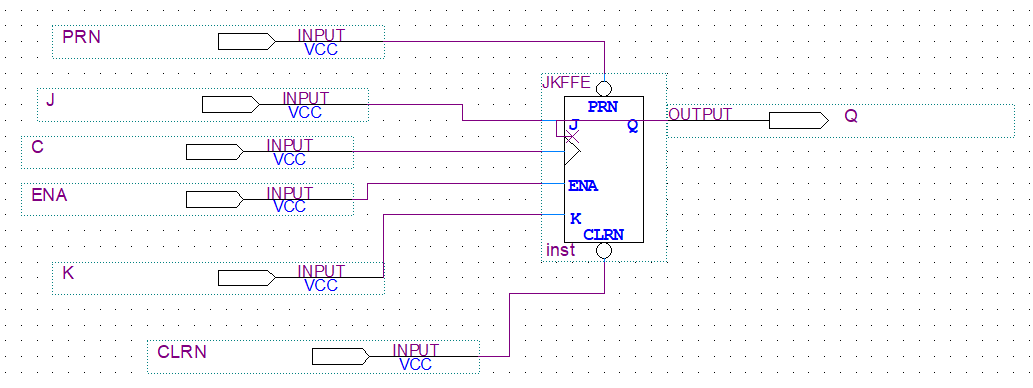
\includegraphics[width=\linewidth]{polytech/scheme/report-lab3/subfiles/images/scheme-4}
		\caption{Разработанная схема триггера}
		\label{fig:scheme-4}
	\end{figure}
    \begin{figure}[H]
		\centering
		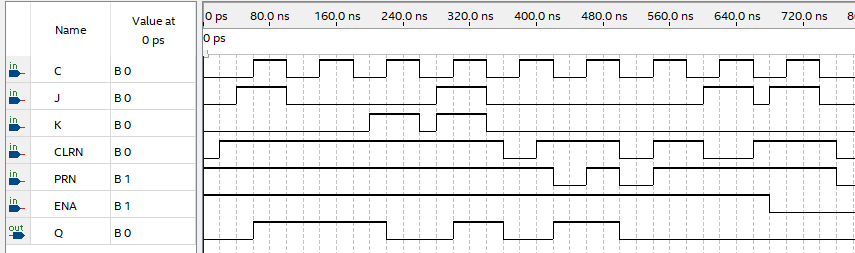
\includegraphics[width=\linewidth]{polytech/scheme/report-lab3/subfiles/images/wave-4}
		\caption{Временная диаграмма}
		\label{fig:wave-4}
	\end{figure}
    При одновременной подаче активного уровня на входы PRN и CLRN триггер устанавливается в 0.
    \subsection{Генератор коротких импульсов}
    \begin{figure}[H]
		\centering
		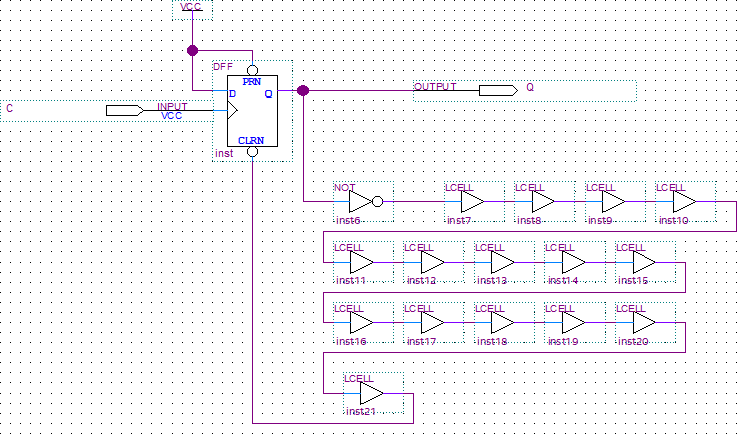
\includegraphics[width=\linewidth]{polytech/scheme/report-lab3/subfiles/images/scheme-5}
		\caption{Разработанная схема триггера}
		\label{fig:scheme-5}
	\end{figure}
    
    Устанавливая элементы LCELL, получаем длительность формируемого импульса в 8 нс. Всего потребовалось
    15 элементов. Разница в примерно 8 нс можно увидеть в значении графы <<Master Time Bar>> на рисунках
    ниже.

    \begin{minipage}{0.49\linewidth}
        \begin{figure}[H]
            \centering
            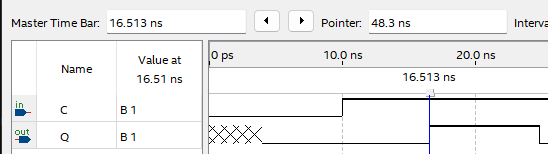
\includegraphics[width=\linewidth]{polytech/scheme/report-lab3/subfiles/images/wave-5-1}
            \caption{Временная диаграмма}
            \label{fig:wave-5-1}
        \end{figure}
    \end{minipage}
    \begin{minipage}{0.49\linewidth}
        \begin{figure}[H]
            \centering
            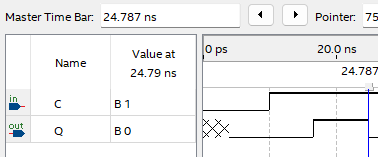
\includegraphics[width=\linewidth]{polytech/scheme/report-lab3/subfiles/images/wave-5-2}
            \caption{Временная диаграмма}
            \label{fig:wave-5-2}
        \end{figure}
    \end{minipage}

    Используя Chip Planner, посмотрим на расположение данной схемы на кристалле и функциональным преобразователем. 
    \begin{figure}[H]
		\centering
		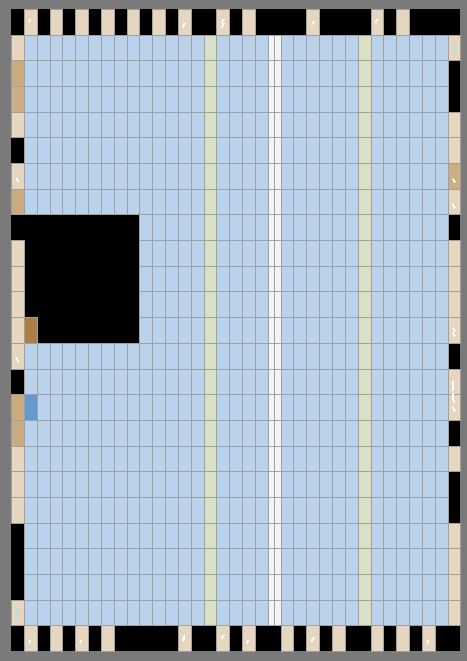
\includegraphics[width=0.38\linewidth]{polytech/scheme/report-lab3/subfiles/images/crystal}
		\caption{Размещение на кристалле}
		\label{fig:crystal}
	\end{figure}
    \begin{figure}[H]
		\centering
		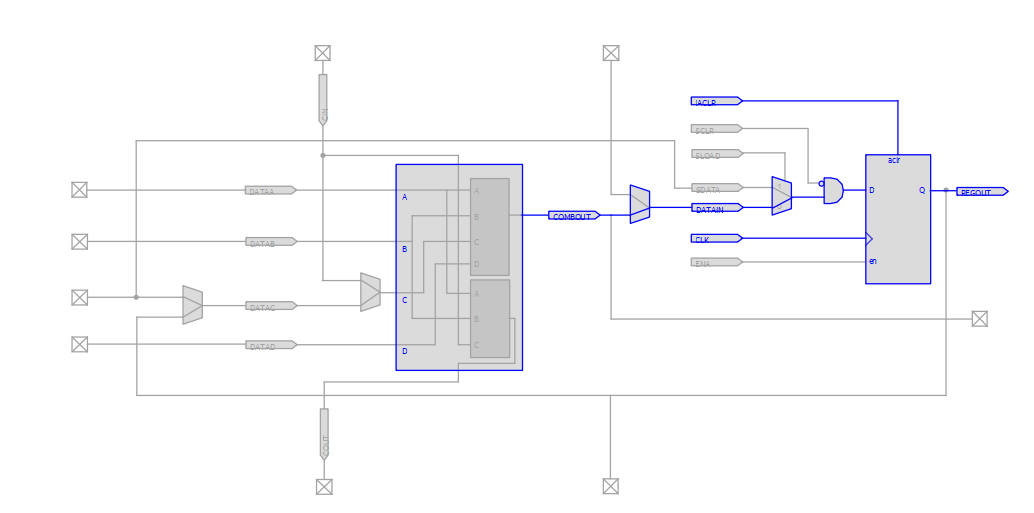
\includegraphics[width=\linewidth]{polytech/scheme/report-lab3/subfiles/images/func_trans}
		\caption{Функциональный преобразователь}
		\label{fig:func_trans}
	\end{figure}

    \subsection{Устройство удвоения частоты}
    Для создания подобного устройства объединим 2 схемы из предыдущего пункта хода работы.
    Один триггер будет формировать единичный импульс при фронте C, а другой при спаде.
    \begin{figure}[H]
		\centering
		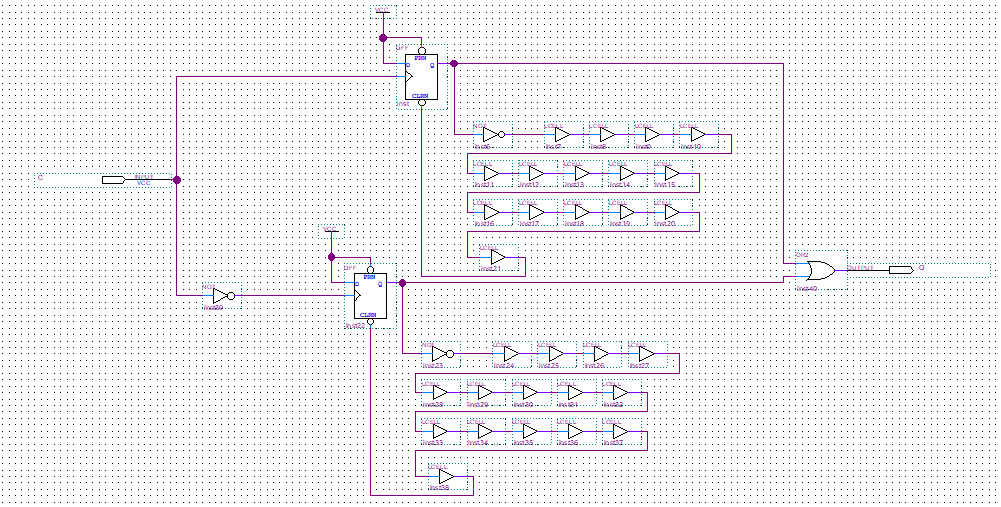
\includegraphics[width=0.9\linewidth]{polytech/scheme/report-lab3/subfiles/images/scheme-7}
		\caption{Разработанная схема устройства}
		\label{fig:scheme-7}
	\end{figure}
    На временной диаграмме видим формирование импульсов как на фронте, так и на спаде.
    \begin{figure}[H]
		\centering
		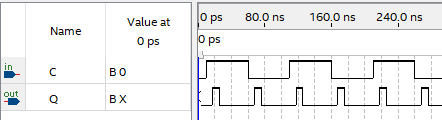
\includegraphics[width=0.9\linewidth]{polytech/scheme/report-lab3/subfiles/images/wave-7}
		\caption{Временная диаграмма}
		\label{fig:wave-7}
	\end{figure}

    \subsection{Устройство выявления спада}
    Для выявления спада сигнала необходимо смотреть на результат логической функции $\overline{D} \cdot Q$.
    \begin{figure}[H]
		\centering
		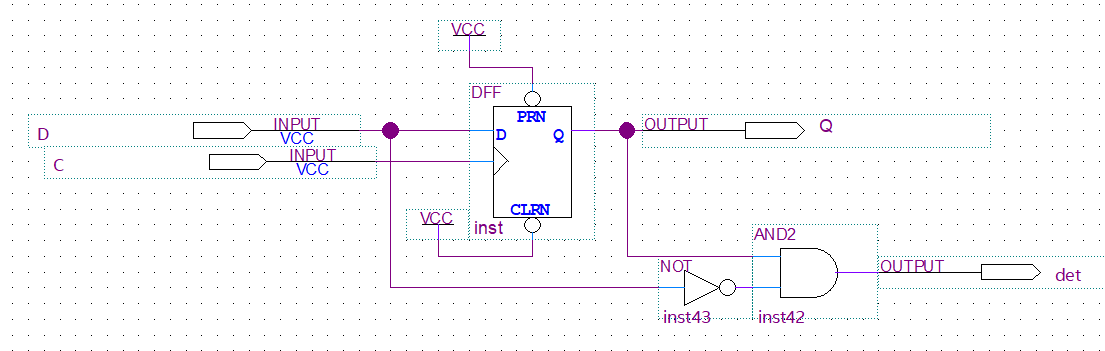
\includegraphics[width=\linewidth]{polytech/scheme/report-lab3/subfiles/images/scheme-8}
		\caption{Разработанная схема устройства}
		\label{fig:scheme-8}
	\end{figure}
    \begin{figure}[H]
		\centering
		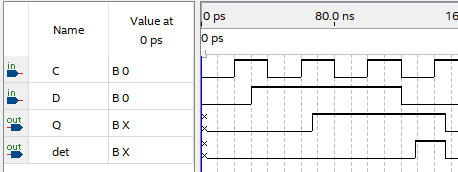
\includegraphics[width=\linewidth]{polytech/scheme/report-lab3/subfiles/images/wave-8}
		\caption{Временная диаграмма}
		\label{fig:wave-8}
	\end{figure}

    \section{Вывод}
    В ходе выполнения работы были закреплены знания характеристик и режимов работы триггеров основных типов.
    Были получены практические навыки тестирования и управления триггерами. Была проведена экспериментальная
    проверка работы типовых устройств с триггерами.
\end{document}
